\chapter{Théorie du champ des ligands et couleur}\label{ch:b2:ligand-field}

Le rubis est rouge et l'émeraude verte, et pourtant tous deux doivent leur couleur au même ion,
\ce{Cr^3+}, dont quelques-uns remplacent l'aluminium dans le corindon, \ce{Al2O3}, ou dans le
béryl. Les cristaux de sulfate de cuivre sont d'un bleu profond, mais la poudre qui reste après
chauffage est blanche. Dans chaque cas, la couleur vient d'électrons qui sautent
entre des orbitales d dont les atomes environnants ont écarté les énergies ---
d'une quantité qui dépend des atomes qui entourent l'ion et de leur disposition. Ce
chapitre calcule cet éclatement, d'abord avec des charges ponctuelles, puis avec des \omterm{def:b2:diatomic-mos:lcao}{orbitales
moléculaires}~; il explique les couleurs, le magnétisme et la \omterm{def:b2:coordination-complexes:electron-count}{règle des 18 électrons} du
chapitre précédent.

\begin{recall}
\Cref{ch:b2:coordination-complexes}~: configurations $d^n$, géométries, décomptes
d'électrons. \Cref{ch:b2:atomic-orbitals}~: les formes des cinq orbitales d.
\Cref{ch:b2:fragment-orbitals}~: \omterm{def:b2:fragment-orbitals:fragment}{orbitales de fragments}. Le volume de première année~: absorbance,
couleurs complémentaires, électrons célibataires, règle de Hund.
\end{recall}

\begin{omfigure}
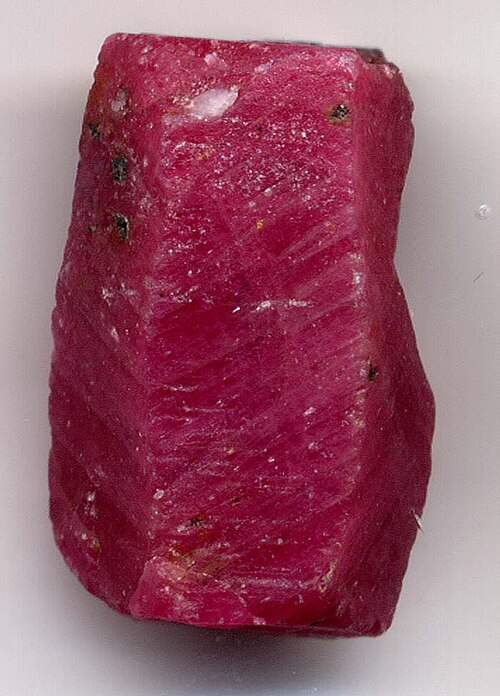
\includegraphics[height=3.6cm]{images/book3/ruby.jpg}\hspace{0.6cm}%
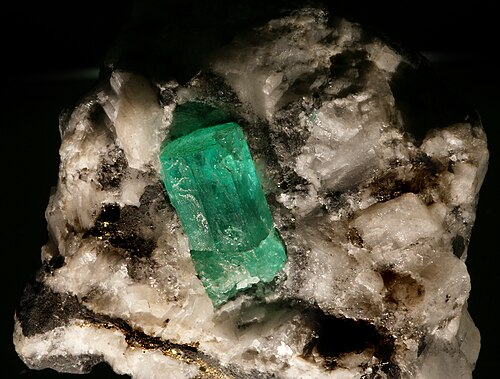
\includegraphics[height=3.6cm]{images/book3/emerald.jpg}\hspace{0.6cm}%
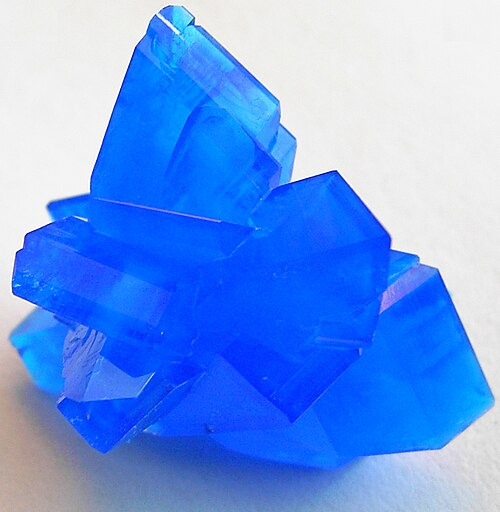
\includegraphics[height=3.6cm]{images/book3/copper-sulfate.jpg}

{\small Un cristal de rubis (domaine public)~; une émeraude dans sa gangue (Didier Descouens,
CC BY-SA 3.0)~; cristaux de sulfate de cuivre(II) pentahydraté (Stephanb, CC BY-SA
3.0). Wikimedia Commons. Le chrome(III) colore les deux premiers, l'aquacomplexe du
cuivre(II) le troisième.}
\end{omfigure}

\section{Le modèle du champ cristallin}

\begin{definition}[Champ cristallin]\label{def:b2:ligand-field:crystal-field}
Le \emph{modèle du champ cristallin}\index{modele du champ cristallin@modèle du champ cristallin} traite les ligands d'un
complexe comme des charges ponctuelles négatives (ou comme les extrémités négatives de dipôles) entourant l'ion
métallique, et calcule comment elles modifient les énergies de ses orbitales d. Dans un champ
octaédrique, les orbitales d se séparent en deux ensembles séparés par l'\emph{éclatement du champ
cristallin}\index{eclatement du champ cristallin@éclatement du champ cristallin} $\Delta_o$.
\end{definition}

Plaçons les six ligands sur les axes. Les orbitales $\mathrm d_{z^2}$ et $\mathrm d_{x^2-y^2}$
dirigent leurs lobes droit sur les ligands~: un électron qui les occupe est davantage repoussé,
et elles montent. Les orbitales $\mathrm d_{xy}$, $\mathrm d_{xz}$, $\mathrm d_{yz}$ pointent entre
les ligands et montent moins. La première paire est appelée $e_g$, le second ensemble de trois
$t_{2g}$ (noms issus de la théorie des groupes, vue dans le volume de troisième année).

\begin{omfigure}
\begin{tikzpicture}[font=\small]
  \begin{scope}
    \pic at (0,0) {omdx2y2};
    \foreach \p in {(1.25,0),(-1.25,0),(0,1.25),(0,-1.25)} \node[circle, fill=black!70, inner sep=2.2pt] at \p {};
    \node at (0,-1.75) {$\mathrm d_{x^2-y^2}$~: lobes vers les ligands};
  \end{scope}
  \begin{scope}[xshift=5.5cm]
    \pic at (0,0) {omdxy};
    \foreach \p in {(1.25,0),(-1.25,0),(0,1.25),(0,-1.25)} \node[circle, fill=black!70, inner sep=2.2pt] at \p {};
    \node at (0,-1.75) {$\mathrm d_{xy}$~: lobes entre eux};
  \end{scope}
\end{tikzpicture}

{\small Deux orbitales d parmi les quatre ligands du plan $xy$ d'un octaèdre
(points noirs). Les lobes de $\mathrm d_{x^2-y^2}$ pointent vers les ligands, ceux de
$\mathrm d_{xy}$ entre eux.}
\end{omfigure}

\begin{theorem}[Barycentre]\label{thm:b2:ligand-field:barycentre}
Dans un champ octaédrique, mesurées à partir de l'énergie moyenne des orbitales d, la
paire $e_g$ se situe à $+0.6\Delta_o$ et l'ensemble $t_{2g}$ à $-0.4\Delta_o$.
\end{theorem}

\begin{proof}
Le champ élève la moyenne des cinq énergies d mais l'éclatement ne la modifie pas
(règle du barycentre, admise~: la somme des déplacements d'un ensemble complet
d'orbitales est fixée par la charge totale, et non par sa disposition). Avec $e_g$ en $x$ et
$t_{2g}$ en $x - \Delta_o$, la condition $2x + 3(x - \Delta_o) = 0$ donne $x = 0.6\Delta_o$.
\end{proof}

\section{Haut spin et bas spin}

\begin{definition}[États de spin]\label{def:b2:ligand-field:spin}
L'\emph{énergie d'appariement}\index{energie d'appariement@énergie d'appariement} $P$ est l'énergie nécessaire pour placer un second
électron dans une orbitale occupée plutôt que dans une orbitale vide de même énergie. Un
complexe est \emph{haut spin}\index{haut spin} lorsque ses électrons occupent les orbitales $e_g$
avant de s'apparier dans $t_{2g}$, \emph{bas spin}\index{bas spin} lorsqu'ils s'apparient d'abord dans $t_{2g}$.
\end{definition}

\begin{proposition}[Choix de l'état de spin]\label{prop:b2:ligand-field:spin-state}
Pour les ions octaédriques $d^4$ à $d^7$, le complexe est \omterm{def:b2:ligand-field:spin}{bas spin} si $\Delta_o > P$ et \omterm{def:b2:ligand-field:spin}{haut spin}
si $\Delta_o < P$. Pour $d^1$--$d^3$ et $d^8$--$d^{10}$, une seule configuration existe.
\end{proposition}

\begin{proof}
À partir de $d^3$ ($t_{2g}^3$), le quatrième électron entre soit dans $e_g$ (coût $\Delta_o$ au-dessus de
$t_{2g}$), soit s'apparie dans $t_{2g}$ (coût $P$). Le moins coûteux l'emporte~; la même comparaison vaut
pour chaque électron jusqu'à $d^7$. Pour $d^1$--$d^3$, il y a de la place dans $t_{2g}$ sans appariement~;
pour $d^8$--$d^{10}$, $t_{2g}$ est plein et $e_g$ doit être utilisé de toute façon.
\end{proof}

\begin{definition}[Énergie de stabilisation du champ cristallin]\label{def:b2:ligand-field:cfse}
L'\emph{énergie de stabilisation du champ cristallin}\index{energie de stabilisation du champ cristallin@énergie de stabilisation du champ cristallin}
(ESCC) d'une configuration $t_{2g}^ae_g^b$ vaut $(-0.4a + 0.6b)\Delta_o$, l'énergie des
électrons d par rapport au barycentre (les \omterm{def:b2:ligand-field:spin}{énergies d'appariement} étant comptées à part).
\end{definition}

\begin{proposition}[L'ESCC le long de la série]\label{prop:b2:ligand-field:cfse}
En \omterm{def:b2:ligand-field:spin}{haut spin}, l'ESCC vaut $0$, $-0.4$, $-0.8$, $-1.2$, $-0.6$, $0$, $-0.4$, $-0.8$, $-1.2$,
$-0.6$, $0$ (en $\Delta_o$) pour $d^0$ à $d^{10}$~: elle s'annule pour $d^0$, $d^5$, $d^{10}$. En \omterm{def:b2:ligand-field:spin}{bas
spin}, elle atteint $-2.4\Delta_o$ pour $d^6$.
\end{proposition}

\begin{proof}
Remplir les configurations et appliquer la définition~; les valeurs sont celles de la figure,
calculées.
\end{proof}

\begin{omfigure}
\begin{tikzpicture}
\begin{axis}[width=0.55\linewidth, height=5cm, xmin=-0.5, xmax=10.5, ymin=-2.6, ymax=0.3,
  axis x line=bottom, axis y line=left, xlabel={$d^n$}, ylabel={ESCC ($\Delta_o$)},
  xtick={0,1,2,3,4,5,6,7,8,9,10}, tick label style={font=\small}, label style={font=\small}]
\addplot[omThm, thick, mark=*, mark size=1.3pt] table[x=n, y=high] {figdata/out/bachelor-2-ligand-field-a.dat};
\addplot[omDef, thick, dashed, mark=square*, mark size=1.3pt] table[x=n, y=low] {figdata/out/bachelor-2-ligand-field-a.dat};
\node[font=\scriptsize, omThm, anchor=west] at (axis cs:5.4,0.0) {haut spin};
\node[font=\scriptsize, omDef, anchor=west] at (axis cs:6.6,-2.2) {bas spin};
\end{axis}
\end{tikzpicture}\hfill
\begin{tikzpicture}[font=\small]
  \pic (t) at (0,0) {omlevel={ud}{0.5}}; \pic at (0.6,0) {omlevel={u}{0.5}}; \pic at (1.2,0) {omlevel={u}{0.5}};
  \pic at (0.3,1.6) {omlevel={u}{0.5}}; \pic at (0.9,1.6) {omlevel={u}{0.5}};
  \node at (0.6,-0.8) {$d^6$ haut spin};
  \node[font=\scriptsize, anchor=east] at (-0.35,0) {$t_{2g}$}; \node[font=\scriptsize, anchor=east] at (-0.05,1.6) {$e_g$};
  \pic at (3,0) {omlevel={ud}{0.5}}; \pic at (3.6,0) {omlevel={ud}{0.5}}; \pic at (4.2,0) {omlevel={ud}{0.5}};
  \pic at (3.3,2.4) {omlevel={empty}{0.5}}; \pic at (3.9,2.4) {omlevel={empty}{0.5}};
  \node at (3.6,-0.8) {$d^6$ bas spin};
  \draw[<->, omProp] (4.7,0) -- (4.7,2.4) node[midway, right, font=\scriptsize] {$\Delta_o$};
  \draw[<->, omProp] (1.7,0) -- (1.7,1.6) node[midway, right, font=\scriptsize] {$\Delta_o$};
\end{tikzpicture}

{\small À gauche~: \omterm{def:b2:ligand-field:cfse}{énergie de stabilisation du champ cristallin} le long de la série d (calculée),
en \omterm{def:b2:ligand-field:spin}{haut spin} (trait plein) et en \omterm{def:b2:ligand-field:spin}{bas spin} (tirets). À droite~: les deux configurations d'un ion $d^6$~:
quatre électrons célibataires lorsque $\Delta_o < P$ (comme \ce{[Fe(H2O)6]^2+}), aucun lorsque $\Delta_o >
P$ (comme \ce{[Fe(CN)6]^4-}).}
\end{omfigure}

\begin{method}[État de spin, ESCC et électrons célibataires]\label{met:b2:ligand-field:spin-state}
\begin{enumerate}
  \item Trouver $n$ à partir du degré d'oxydation ($n = g - m$).
  \item Pour $d^4$--$d^7$, comparer $\Delta_o$ et $P$ (ou situer le ligand dans la
        \omterm{def:b2:ligand-field:spectrochemical}{série spectrochimique})~: champ fort, \omterm{def:b2:ligand-field:spin}{bas spin}~; champ faible, \omterm{def:b2:ligand-field:spin}{haut spin}.
  \item Remplir $t_{2g}$ et $e_g$ en conséquence~; ESCC $= (-0.4a + 0.6b)\Delta_o$.
  \item Compter les électrons célibataires~; tout électron célibataire rend le complexe
        \omterm{def:b2:diatomic-mos:magnetism}{paramagnétique}.
\end{enumerate}
\end{method}

\section{Autres géométries}

\begin{proposition}[Champs tétraédrique et plan carré]\label{prop:b2:ligand-field:tetrahedral}
Dans un champ tétraédrique, l'ordre est inversé~: deux orbitales ($e$) au-dessous de trois ($t_2$),
avec un éclatement $\Delta_t \approx \frac49\Delta_o$ pour le même métal et les mêmes ligands~; les complexes
tétraédriques sont \omterm{def:b2:ligand-field:spin}{haut spin}. Dans un champ plan carré, l'orbitale $\mathrm d_{x^2-y^2}$ se situe très
au-dessus des autres~: un ion $d^8$ remplit les quatre orbitales inférieures et la laisse vide.
\end{proposition}

\admitted

Le facteur $4/9$ vient de la géométrie des charges ponctuelles~; avec quatre ligands seulement,
dont aucun ne pointe selon les axes, l'éclatement est trop faible pour vaincre l'\omterm{def:b2:ligand-field:spin}{énergie
d'appariement}. Retirer les deux ligands de l'axe $z$ d'un octaèdre abaisse les orbitales qui ont
une composante selon $z$ et n'élève rien~: cela explique les complexes $d^8$ plans carrés du
chapitre précédent, dont les huit électrons trouvent tous place au-dessous de l'orbitale vide
$\mathrm d_{x^2-y^2}$.

\begin{omfigure}
\begin{tikzpicture}[font=\scriptsize]
  % octahedral
  \pic at (-0.3,0) {omlevel={empty}{0.45}}; \pic at (0.25,0) {omlevel={empty}{0.45}}; \pic at (0.8,0) {omlevel={empty}{0.45}};
  \pic at (0,1.8) {omlevel={empty}{0.45}}; \pic at (0.55,1.8) {omlevel={empty}{0.45}};
  \node[anchor=west] at (1.1,0) {$t_{2g}$}; \node[anchor=west] at (0.85,1.8) {$e_g$};
  \node[font=\small] at (0.25,-0.7) {octaédrique};
  % tetrahedral
  \begin{scope}[xshift=3.5cm]
    \pic at (0,0.6) {omlevel={empty}{0.45}}; \pic at (0.55,0.6) {omlevel={empty}{0.45}};
    \pic at (-0.3,1.4) {omlevel={empty}{0.45}}; \pic at (0.25,1.4) {omlevel={empty}{0.45}}; \pic at (0.8,1.4) {omlevel={empty}{0.45}};
    \node[anchor=west] at (0.85,0.6) {$e$}; \node[anchor=west] at (1.1,1.4) {$t_2$};
    \node[font=\small] at (0.25,-0.7) {tétraédrique};
  \end{scope}
  % square planar
  \begin{scope}[xshift=7cm]
    \pic at (0,-0.2) {omlevel={empty}{0.45}}; \pic at (0.55,-0.2) {omlevel={empty}{0.45}};
    \pic at (0.25,0.3) {omlevel={empty}{0.45}};
    \pic at (0.25,0.9) {omlevel={empty}{0.45}};
    \pic at (0.25,2.6) {omlevel={empty}{0.45}};
    \node[anchor=west] at (0.85,-0.2) {$\mathrm d_{xz}, \mathrm d_{yz}$};
    \node[anchor=west] at (0.55,0.3) {$\mathrm d_{z^2}$};
    \node[anchor=west] at (0.55,0.9) {$\mathrm d_{xy}$};
    \node[anchor=west] at (0.55,2.6) {$\mathrm d_{x^2-y^2}$};
    \node[font=\small] at (0.25,-0.7) {plan carré};
  \end{scope}
\end{tikzpicture}

{\small Éclatement des orbitales d dans trois géométries, schéma (pas à la même
échelle)~: octaédrique, tétraédrique (inversé et plus petit), plan carré (une orbitale très
au-dessus des autres).}
\end{omfigure}

\section{Couleur et série spectrochimique}

\begin{definition}[Transition d--d]\label{def:b2:ligand-field:d-d}
Une \emph{transition d--d}\index{transition d--d} est la promotion d'un électron d'un
niveau d inférieur vers un niveau d supérieur d'un complexe par absorption de lumière~; pour un ion $d^1$, de
$t_{2g}$ vers $e_g$, à l'énergie $\Delta_o$.
\end{definition}

\begin{proposition}[L'éclatement d'après la couleur]\label{prop:b2:ligand-field:colour}
Si un complexe absorbe le plus fortement à la longueur d'onde $\lambda_{\max}$ par une \omterm{def:b2:ligand-field:d-d}{transition d--d}
d'énergie $\Delta_o$, alors $\Delta_o = N_Ahc/\lambda_{\max}$ par mole, ou $\tilde\nu = 1/\lambda_{\max}$
en nombre d'onde~; la couleur perçue est la complémentaire de la couleur absorbée.
\end{proposition}

\begin{proof}
Un photon de longueur d'onde $\lambda$ transporte $hc/\lambda$~; une mole de photons, $N_Ahc/\lambda$. La lumière
blanche privée de la bande absorbée apparaît de la couleur complémentaire.
\end{proof}

\begin{method}[D'une bande d'absorption à une couleur]\label{met:b2:ligand-field:colour}
\begin{enumerate}
  \item Convertir $\lambda_{\max}$ en $\tilde\nu = 1/\lambda_{\max}$ (\unit{cm^{-1}}) et en
        $N_Ahc/\lambda_{\max}$ (\unit{kJ/mol})~: $\qty{500}{nm} \leftrightarrow \qty{20000}{cm^{-1}}
        \leftrightarrow \qty{239}{kJ/mol}$.
  \item Trouver la couleur absorbée (violet 400--430, bleu 430--490, vert 490--560, jaune
        560--590, orange 590--620, rouge 620--700 nm, approximativement).
  \item La couleur perçue est opposée sur le cercle chromatique.
\end{enumerate}
\end{method}

\begin{omfigure}
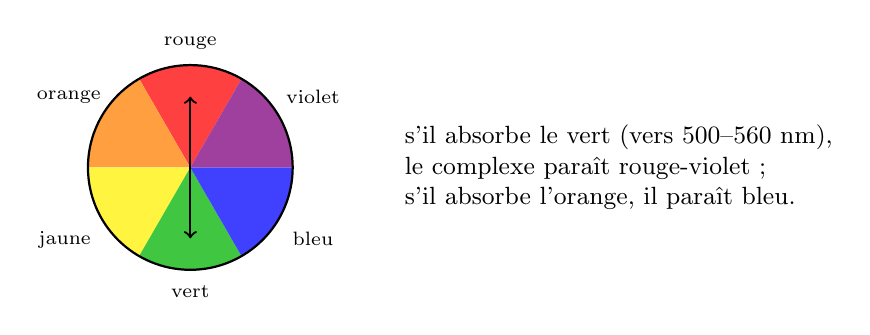
\begin{tikzpicture}[font=\scriptsize]
  \foreach \a/\c/\n in {90/red/rouge, 150/orange/orange, 210/yellow/jaune, 270/green!70!black/vert, 330/blue/bleu, 30/violet/violet} {
    \fill[\c!75] (0,0) -- (\a-30:1.3) arc[start angle=\a-30, end angle=\a+30, radius=1.3] -- cycle;
    \node[anchor=\a+180] at (\a:1.38) {\n};
  }
  \draw[thick] (0,0) circle (1.3);
  \draw[<->, thick] (90:0.9) -- (270:0.9);
  \node[anchor=west, font=\small, align=left] at (2.6,0) {s'il absorbe le vert (vers 500--560 nm),\\ le complexe paraît rouge-violet~;\\ s'il absorbe l'orange, il paraît bleu.};
\end{tikzpicture}

{\small Un cercle chromatique~: la couleur perçue est à peu près la complémentaire, diamétralement
opposée, de la bande absorbée.}
\end{omfigure}

\begin{definition}[Série spectrochimique]\label{def:b2:ligand-field:spectrochemical}
La \emph{série spectrochimique}\index{serie spectrochimique@série spectrochimique} classe les ligands selon
l'éclatement qu'ils produisent pour un ion métallique donné~:
\[
  \ce{I-} < \ce{Br-} < \ce{Cl-} < \ce{F-} < \ce{OH-} < \ce{H2O} < \ce{NH3} < \text{en} <
  \ce{NO2-} < \ce{CN-} < \ce{CO} .
\]
Pour un ligand donné, $\Delta_o$ croît aussi avec la charge de l'ion métallique et en descendant un groupe
(les complexes 4d et 5d, plus étendus que les 3d, sont presque toujours \omterm{def:b2:ligand-field:spin}{bas spin}).
\end{definition}

Les halogénures sont à l'extrémité faible et \ce{CN-} et \ce{CO} à l'extrémité forte, ce que le
\omterm{def:b2:ligand-field:crystal-field}{modèle du champ cristallin} ne peut pas expliquer~: il placerait l'ion chargé \ce{F-} au-dessus de la molécule neutre
\ce{CO}. L'explication exige des orbitales.

\section{Le champ des ligands}

\begin{definition}[Théorie du champ des ligands]\label{def:b2:ligand-field:ligand-field}
La \emph{théorie du champ des ligands}\index{theorie du champ des ligands@théorie du champ des ligands} décrit un complexe par des \omterm{def:b2:diatomic-mos:lcao}{orbitales moléculaires}
construites à partir des orbitales de valence du métal (ses neuf orbitales $n$d, $(n+1)$s et $(n+1)$p)
et des orbitales donneuses des ligands.
\end{definition}

\begin{proposition}[Liaison $\sigma$ dans un complexe octaédrique]\label{prop:b2:ligand-field:mo-octahedral}
Avec six ligands apportant chacun une orbitale $\sigma$ donneuse, six \omterm{def:b2:diatomic-mos:lcao}{orbitales moléculaires} liantes se forment
à partir de l'orbitale s du métal, de ses trois p et de ses deux orbitales d $e_g$~; les trois orbitales $t_{2g}$, qui
pointent entre les ligands, restent non liantes~; au-dessus d'elles se trouvent les \omterm{def:b2:diatomic-mos:bonding}{orbitales antiliantes} $e_g^*$.
Les électrons des ligands remplissent les six \omterm{def:b2:diatomic-mos:bonding}{orbitales liantes}~; les électrons d du métal vont
dans $t_{2g}$ et $e_g^*$, séparées par $\Delta_o$. Les \omterm{def:b2:diatomic-mos:bonding}{orbitales liantes} et non liantes peuvent contenir
$12 + 6 = 18$ électrons.
\end{proposition}

\begin{proof}[Argument]
Par la méthode des fragments du \cref{ch:b2:fragment-orbitals}, chaque orbitale du métal interagit
avec la combinaison d'orbitales des ligands de même symétrie~: s avec la combinaison totalement
symétrique, chaque p avec une paire de ligands opposés, $\mathrm d_{z^2}$ et $\mathrm
d_{x^2-y^2}$ avec les combinaisons dirigées selon leurs lobes~; aucune combinaison $\sigma$
ne correspond aux orbitales $t_{2g}$ (leur recouvrement avec tout donneur $\sigma$ dirigé selon un axe
est nul par symétrie). Les noms des combinaisons viennent de la théorie des groupes, admise.
Remplir toutes les \omterm{def:b2:diatomic-mos:bonding}{orbitales liantes} et non liantes, et aucune antiliante, demande
18 électrons --- c'est la \omterm{def:b2:coordination-complexes:electron-count}{règle des 18 électrons}.
\end{proof}

\begin{omfigure}
\begin{tikzpicture}[font=\scriptsize]
  % metal
  \pic (m4p1) at (-0.45,2.6) {omlevel={empty}{0.4}}; \pic (m4p2) at (0,2.6) {omlevel={empty}{0.4}}; \pic (m4p3) at (0.45,2.6) {omlevel={empty}{0.4}};
  \node[anchor=east] at (-0.7,2.6) {$(n{+}1)$p};
  \pic (m4s) at (0,1.8) {omlevel={empty}{0.6}}; \node[anchor=east] at (-0.35,1.8) {$(n{+}1)$s};
  \foreach \x in {-0.9,-0.45,0,0.45,0.9} \pic at (\x,0.6) {omlevel={empty}{0.4}};
  \coordinate (m3d) at (1.1,0.6); \node[anchor=east] at (-1.15,0.6) {$n$d};
  \node[font=\small] at (0,-2.9) {métal};
  % ligands
  \foreach \x in {6.2,6.72,7.24,7.76,8.28,8.8} \pic at (\x,-0.9) {omlevel={ud}{0.36}};
  \coordinate (lig) at (6.0,-0.9);
  \node[font=\small] at (7.3,-2.9) {six orbitales $\sigma$ donneuses};
  % MOs
  \pic (b1) at (3.6,-2.4) {omlevel={ud}{0.5}};
  \foreach \x in {3.0,3.6,4.2} \pic at (\x,-1.9) {omlevel={ud}{0.5}};
  \pic at (3.3,-1.45) {omlevel={ud}{0.5}}; \pic at (3.9,-1.45) {omlevel={ud}{0.5}};
  \foreach \x in {3.0,3.6,4.2} \pic at (\x,0.3) {omlevel={empty}{0.5}};
  \pic at (3.3,1.5) {omlevel={empty}{0.5}}; \pic at (3.9,1.5) {omlevel={empty}{0.5}};
  \pic at (3.6,3.1) {omlevel={empty}{0.5}};
  \foreach \x in {3.0,3.6,4.2} \pic at (\x,3.6) {omlevel={empty}{0.5}};
  \node[anchor=north] at (3.6,0.12) {$t_{2g}$ (non liantes)};
  \node[anchor=west] at (4.2,1.5) {$e_g^*$};
  \node[anchor=north] at (3.6,-2.58) {6 liantes};
  \draw[<->, omProp] (2.55,0.3) -- (2.55,1.5) node[midway, right] {$\Delta_o$};
  \draw[omcorr, densely dashed] (m3d) -- (2.75,0.3) (m3d) -- (3.05,1.5) (1.1,0.6) -- (3.05,-1.45);
  \draw[omcorr, densely dashed] (lig) -- (4.15,-1.45) (lig) -- (4.45,-1.9) (lig) -- (3.85,-2.4) (lig) -- (4.15,1.5);
  \draw[omcorr, densely dashed] (m4s-r) -- (3.35,-2.4) (m4s-r) -- (3.35,3.1) (m4p3-r) -- (2.75,-1.9) (m4p3-r) -- (2.75,3.6);
\end{tikzpicture}

{\small \omterm{def:b2:diatomic-mos:lcao}{Orbitales moléculaires} d'un complexe octaédrique à six donneurs $\sigma$,
schéma. Les douze électrons des ligands remplissent les six \omterm{def:b2:diatomic-mos:bonding}{orbitales liantes}~; les électrons d
du métal occupent les niveaux non liants $t_{2g}$ et antiliants $e_g^*$, séparés par
$\Delta_o$ --- on retrouve l'image du champ cristallin. Jusqu'à 18 électrons remplissent les niveaux liants et
non liants.}
\end{omfigure}

\begin{definition}[Ligands $\pi$-donneurs et $\pi$-accepteurs]\label{def:b2:ligand-field:pi-ligands}
Un \emph{ligand $\pi$-donneur}\index{ligand pi-donneur@ligand $\pi$-donneur} possède des orbitales pleines
de symétrie $\pi$ par rapport à la liaison métal--ligand (doublets non liants de \ce{Cl-},
\ce{OH-})~; un \emph{ligand $\pi$-accepteur}\index{ligand pi-accepteur@ligand $\pi$-accepteur}
en possède de vides de basse énergie (les orbitales $\pi^*$ de \ce{CO} et de \ce{CN-}). Le transfert de
densité électronique des orbitales d pleines du métal vers les orbitales $\pi^*$ vides d'un
ligand $\pi$-accepteur est appelé \emph{rétrodonation}\index{retrodonation@rétrodonation}.
\end{definition}

\begin{proposition}[Effets $\pi$ sur l'éclatement]\label{prop:b2:ligand-field:pi-effects}
Les ligands $\pi$-donneurs diminuent $\Delta_o$~; les ligands $\pi$-accepteurs l'augmentent.
\end{proposition}

\begin{proof}
Les orbitales $t_{2g}$ ont la bonne symétrie pour recouvrir les orbitales $\pi$ des ligands. Une orbitale $\pi$
pleine du ligand se situe au-dessous de $t_{2g}$~: d'après le \cref{thm:b2:frontier-orbitals:perturbation},
l'interaction repousse $t_{2g}$ vers le haut, vers $e_g^*$, et $\Delta_o$ diminue. Une orbitale $\pi^*$ vide
se situe au-dessus de $t_{2g}$~: l'interaction repousse $t_{2g}$ vers le bas, et $\Delta_o$ augmente. Le second cas
transfère de la densité d du métal vers l'orbitale $\pi^*$ du ligand~: c'est la \omterm{def:b2:ligand-field:pi-ligands}{rétrodonation}.
\end{proof}

\begin{omfigure}
\begin{tikzpicture}[font=\scriptsize]
  \begin{scope}
    \pic (t) at (0,1.2) {omlevel={empty}{0.6}}; \node[anchor=east] at (-0.35,1.2) {$t_{2g}$};
    \pic (l) at (2.4,0) {omlevel={ud}{0.6}}; \node[anchor=west] at (2.75,0) {$\pi$ du ligand (pleine)};
    \pic (n) at (1.2,1.75) {omlevel={empty}{0.6}};
    \draw[omcorr, densely dashed] (t-r) -- (n-l) (l-l) -- (n-r);
    \pic (e) at (1.2,3.0) {omlevel={empty}{0.6}}; \node[anchor=west] at (1.55,3.0) {$e_g^*$};
    \draw[<->, omProp] (0.55,1.75) -- (0.55,3.0) node[midway, left] {$\Delta_o$ plus petit};
    \node[font=\small] at (1.2,-0.8) {donneur $\pi$};
  \end{scope}
  \begin{scope}[xshift=6.5cm]
    \pic (t) at (0,1.2) {omlevel={empty}{0.6}}; \node[anchor=east] at (-0.35,1.2) {$t_{2g}$};
    \pic (l) at (2.4,2.6) {omlevel={empty}{0.6}}; \node[anchor=west] at (2.75,2.6) {$\pi^*$ du ligand (vide)};
    \pic (n) at (1.2,0.65) {omlevel={empty}{0.6}};
    \draw[omcorr, densely dashed] (t-r) -- (n-l) (l-l) -- (n-r);
    \pic (e) at (1.2,3.0) {omlevel={empty}{0.6}}; \node[anchor=west] at (1.55,3.15) {$e_g^*$};
    \draw[<->, omProp] (0.55,0.65) -- (0.55,3.0) node[midway, left] {$\Delta_o$ plus grand};
    \node[font=\small] at (1.2,-0.8) {accepteur $\pi$ (rétrodonation)};
  \end{scope}
\end{tikzpicture}

{\small Effet des orbitales $\pi$ des ligands sur le niveau $t_{2g}$, schéma. Une orbitale $\pi$ pleine du ligand,
située au-dessous, repousse $t_{2g}$ vers le haut (éclatement plus petit)~; une orbitale $\pi^*$ vide, située au-dessus, l'attire
vers le bas (éclatement plus grand).}
\end{omfigure}

Cela place \ce{CO} et \ce{CN-}, forts donneurs $\sigma$ et accepteurs $\pi$, en haut de la
\omterm{def:b2:ligand-field:spectrochemical}{série spectrochimique}, et les halogénures, donneurs $\pi$, en bas. Les métaux carbonyles ont
leurs orbitales $t_{2g}$ stabilisées et remplies~: ce sont les complexes à 18 électrons du
\cref{ch:b2:coordination-complexes}.

\section{Exercices}

\begin{exercise}[$\star$]\label{exo:b2:ligand-field:1}
Donner la configuration octaédrique et l'ESCC d'un ion $d^3$ et d'un ion $d^8$.
\end{exercise}

\begin{exercise}[$\star$]\label{exo:b2:ligand-field:2}
Combien d'électrons célibataires possèdent \ce{[Fe(H2O)6]^2+} (\omterm{def:b2:ligand-field:spin}{haut spin}) et \ce{[Fe(CN)6]^4-} (\omterm{def:b2:ligand-field:spin}{bas
spin})~?
\end{exercise}

\begin{exercise}[$\star$]\label{exo:b2:ligand-field:3}
Un complexe absorbe le plus fortement à \qty{600}{nm}. De quelle couleur paraît-il~?
\end{exercise}

\begin{exercise}[$\star$]\label{exo:b2:ligand-field:4}
Classer \ce{H2O}, \ce{CN-}, \ce{Cl-}, \ce{NH3} selon l'éclatement qu'ils produisent.
\end{exercise}

\begin{exercise}[$\star\star$]\label{exo:b2:ligand-field:5}
Pour un ion $d^5$, $\Delta_o = \qty{165}{kJ/mol}$ avec l'eau et $\qty{390}{kJ/mol}$ avec le cyanure,
et $P = \qty{300}{kJ/mol}$ (données de l'exercice). Prévoir les deux états de spin et les électrons
célibataires.
\end{exercise}

\begin{exercise}[$\star\star$]\label{exo:b2:ligand-field:6}
\ce{[Co(H2O)6]^2+} est rose, \ce{[CoCl4]^2-} d'un bleu profond. Expliquer le changement de couleur par le
changement de géométrie et de ligand.
\end{exercise}

\begin{exercise}[$\star\star$]\label{exo:b2:ligand-field:7}
Montrer que le complexe plan carré \ce{[Ni(CN)4]^2-} est \omterm{def:b2:diatomic-mos:magnetism}{diamagnétique}, alors que le complexe tétraédrique
\ce{[NiCl4]^2-} possède deux électrons célibataires.
\end{exercise}

\begin{exercise}[$\star\star$]\label{exo:b2:ligand-field:8}
Un complexe $d^1$ absorbe à \qty{500}{nm} (données de l'exercice). Calculer $\Delta_o$ en \unit{cm^{-1}} et
en \unit{kJ/mol}.
\end{exercise}

\begin{exercise}[$\star\star$]\label{exo:b2:ligand-field:9}
Pourquoi les composés de \ce{Zn^2+} et de \ce{Sc^3+} sont-ils incolores~?
\end{exercise}

\begin{exercise}[$\star\star\star$]\label{exo:b2:ligand-field:10}
Compter les électrons dans les \omterm{def:b2:diatomic-mos:lcao}{orbitales moléculaires} de \ce{[Co(NH3)6]^3+}~: quels niveaux sont remplis,
et le complexe est-il \omterm{def:b2:diatomic-mos:magnetism}{diamagnétique}~?
\end{exercise}

\begin{exercise}[$\star\star\star$]\label{exo:b2:ligand-field:11}
Expliquer pourquoi \ce{CO}, molécule neutre et faiblement basique, produit un éclatement plus grand que
l'ion fluorure.
\end{exercise}

\begin{exercise}[$\star\star\star$]\label{exo:b2:ligand-field:12}
Les enthalpies d'hydratation des ions \ce{M^2+} de \ce{Ca^2+} à \ce{Zn^2+}, tracées en fonction de $n$, forment
deux bosses au-dessus d'une droite passant par $d^0$, $d^5$ et $d^{10}$. Expliquer cette allure par
l'ESCC en \omterm{def:b2:ligand-field:spin}{haut spin}.
\end{exercise}

\section{Problème~: rubis rouge, émeraude verte}

\begin{problem}[{Problème du week-end --- le chrome(III) dans un champ octaédrique, les bandes
d'absorption du rubis et la couleur qu'elles laissent, le champ plus faible de l'émeraude, et le sulfate
de cuivre hydraté et anhydre}]
\label{pb:b2:ligand-field:1}
Données fixées pour le problème (arrondies, à titre d'illustration)~: le rubis (\ce{Cr^3+} dans \ce{Al2O3}) absorbe
dans deux bandes, vers \qty{556}{nm} et \qty{405}{nm}~; dans l'émeraude (\ce{Cr^3+} dans le béryl), la
première bande se situe vers \qty{620}{nm}. Pour un ion $d^3$, la première bande correspond à
$\Delta_o$. $N_Ahc = \qty{0.1196}{J.m/mol}$.
% ledger: const:NA, const:h, const:c

\medskip
\noindent\textbf{Partie I --- Le chrome(III).}
\begin{enumerate}
  \item Donner la configuration $d^n$ de \ce{Cr^3+}.
  \item Comment se répartit-elle dans un champ octaédrique~?
  \item Y a-t-il un choix entre \omterm{def:b2:ligand-field:spin}{haut spin} et \omterm{def:b2:ligand-field:spin}{bas spin}~?
  \item Calculer son ESCC.
  \item Combien d'électrons célibataires possède-t-il~?
  \item Pourquoi les complexes du chrome(III) sont-ils cinétiquement inertes (lents à échanger leurs ligands)~?
\end{enumerate}

\medskip
\noindent\textbf{Partie II --- Le rubis.}
\begin{enumerate}[resume]
  \item Qu'est-ce qui entoure un ion \ce{Cr^3+} substitué à \ce{Al^3+} dans le corindon~?
  \item Convertir la première bande en nombre d'onde.
  \item En déduire $\Delta_o$ en \unit{kJ/mol}.
  \item Quelles couleurs sont absorbées par les deux bandes~?
  \item Que reste-t-il à voir~?
  \item Pourquoi y a-t-il deux bandes pour un seul éclatement~? (Réponse qualitative.)
\end{enumerate}

\medskip
\noindent\textbf{Partie III --- L'émeraude.}
\begin{enumerate}[resume]
  \item Convertir la bande de l'émeraude en $\Delta_o$.
  \item Comparer au rubis~: quel cristal donne le champ le plus fort~?
  \item Où se déplace la couleur absorbée, et quelle couleur est transmise~?
  \item Proposer une raison structurale au champ plus faible dans le béryl.
  \item Le nombre d'électrons célibataires changerait-il~?
\end{enumerate}

\medskip
\noindent\textbf{Partie IV --- Le sulfate de cuivre.}
\begin{enumerate}[resume]
  \item Quelle est la configuration de \ce{Cu^2+}~?
  \item Dans \ce{CuSO4.5H2O}, le cuivre est entouré de molécules d'eau. Pourquoi le solide est-il bleu~?
  \item Qu'advient-il de la couleur quand on chasse l'eau, et pourquoi~?
  \item Pourquoi une goutte d'eau rend-elle bleue la poudre blanche~?
  \item \ce{[Cu(NH3)4]^2+} absorberait-il à plus courte ou à plus grande longueur d'onde que l'aquacomplexe~?
  \item Un ion $d^9$ peut-il être \omterm{def:b2:ligand-field:spin}{haut spin} ou \omterm{def:b2:ligand-field:spin}{bas spin}~?
  \item \ce{CuSO4.5H2O} est-il \omterm{def:b2:diatomic-mos:magnetism}{paramagnétique}~?
  \item Donner le $\Delta_o$ de \ce{Cr^3+} dans le rubis d'après sa première bande d'absorption.
\end{enumerate}
\end{problem}
